% Licensed under the Creative Commons Attribution Share Alike 4.0 International.
% See the LICENSE file in the repository root for full license text.

\section{寄存器}

\subsection{指令指针寄存器}

虚拟内存空间很大;对现代的个人计算机而言,物理内存也不小。但并非所有数据都存放在内存中。CPU 中使用其内部的\textbf{寄存器(register)}保存当前的控制状态和少量数据。回到图 \ref{pic:asm},表示当前正在执行的指令的 \lstinline{>>} 符号应该由谁负责保管?正是指令指针寄存器 IP\footnote{I 表示 Instruction,P 表示 Pointer,故 IP 寄存器的全称为指令指针寄存器。}。图 \ref{pic:ip} 是 IP 寄存器的又一例子。

\begin{figure}[H]
	\centering
	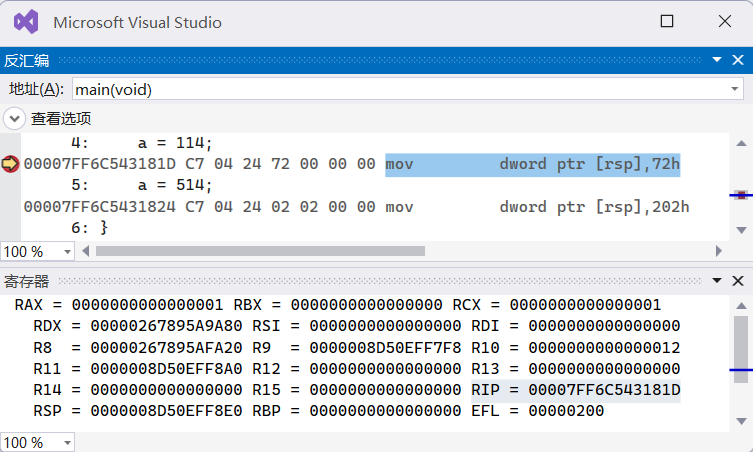
\includegraphics[width=0.7\linewidth]{pic/ip-1.png}
	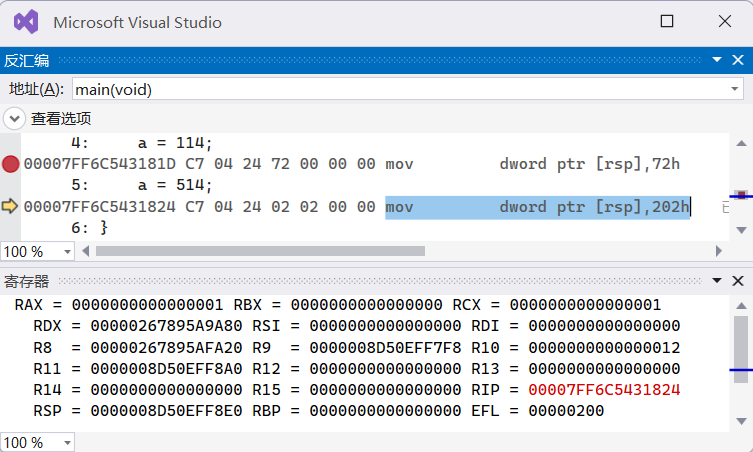
\includegraphics[width=0.7\linewidth]{pic/ip-2.png}
	\caption{IP 寄存器}
	\label{pic:ip}
\end{figure}

图 \ref{pic:ip} 信息丰富。其中的高级语言源代码为:

\begin{lstlisting}[language=c++, numbers=none]
a = 114; // 把 114 放进 a 对应的存储器中。
a = 514; // 把 514 放进 a 对应的存储器中。
\end{lstlisting}

这两句代码各自只对应一条汇编指令:

\begin{lstlisting}[language=assembly, numbers=none]
mov dword ptr [rsp], 72h ; h 后缀表示十六进制。
mov dword ptr [rsp], 202h
\end{lstlisting}

从图 \ref{pic:ip} 可知,这两条指令每条长 7 字节。运行程序时,操作系统将程序代码放入内存中,这两条指令的地址\footnote{注意是虚拟地址。多次运行会有不同的结果。}分别是(十六进制):

\begin{lstlisting}[language={}, numbers=none]
00007FF6C543181D
00007FF6C5431824
\end{lstlisting}

寄存器窗口中的 RIP\footnote{前缀 R 表示这是一个 64 位寄存器。如果是 32 位程序,对应的寄存器名为 EIP,带有前缀 E。16 位的指令指针寄存器就是 IP,没有前缀,但它只能在 16 位计算机上见到。} 即为前文所述的 IP 寄存器。对比地址可知,\textbf{反汇编窗口中的黄色箭头就是 IP 寄存器的替身}。

\begin{note}
	记住这个黄色箭头。我们之后的程序设计不会涉及反汇编和寄存器,但是黄色箭头还会出现。
\end{note}

\subsection{栈指针寄存器}

根据冯·诺依曼计算机“将编制好的程序放入存储器后,首先执行第一条指令,之后周而复始地取出指令、分析指令、执行指令”的工作方式,IP 寄存器是必需的,否则 CPU 不知道该取出哪条指令。但下面提到的栈指针寄存器 SP 对于冯·诺依曼计算机而言并不必要,不过,对现在的程序是不可或缺的。

我们首先了解一下什么是\textbf{栈(stack)}。栈的显著特点是\textbf{先入后出},有如一个只开一端的羽毛球筒,如图 \ref{pic:badminton}\footnote{图源:pphl,《羽毛球航天飞机桶》,Veer 图库,\url{https://www.veer.com/photo/158582104}。仅用作教育用途。} 所示。

\begin{figure}[H]
	\centering
	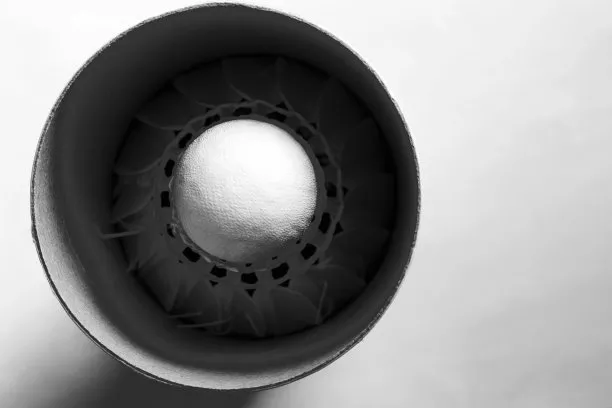
\includegraphics[width=0.4\linewidth]{pic/badminton.png}
	\caption{只开一端的羽毛球筒,忽略把球从这端放入的难度}
	\label{pic:badminton}
\end{figure}

图 \ref{pic:badminton} 中最上面的羽毛球所处的位置被称为\textbf{栈顶(top)},如果栈没有满,则可以把新的羽毛球放到原来的栈顶之上。如果规定一次只能取一个球,则\textbf{只有栈顶处的羽毛球可以被看到和拿出}。相应的,最里面的羽毛球所处的位置被称为\textbf{栈底(bottom)}。如果栈顶和栈底之间没有任何羽毛球,就说明栈空了。

在数据结构领域,栈最重要的用途之一处理括号匹配问题。方法是把左括号看作\textbf{入栈(push)},把右括号看作\textbf{出栈(pop)},然后从左向右处理括号序列,则括号不匹配对应两种情况:

\begin{enumerate}
	\item 在处理过程中出现要求空栈出栈的情况,说明此处右括号多余。
	\item 在处理结束后出现栈非空的情况,说明结尾处左括号多余。
\end{enumerate}

例如,括号序列 \lstinline{(()())} 是匹配的,处理过程为:

\begin{table}[H]
	\centering
	\begin{tabular}{|c|}
		\phantom{(}
		\\\hline
		\\\hline
		\\\hline
	\end{tabular}
	$\stackrel{\text{左}}{\longrightarrow}$
	\begin{tabular}{|c|}
		\phantom{(}
		\\\hline
		\\\hline
		(
		\\\hline
	\end{tabular}
	$\stackrel{\text{左}}{\longrightarrow}$
	\begin{tabular}{|c|}
		\phantom{(}
		\\\hline
		(
		\\\hline
		(
		\\\hline
	\end{tabular}
	$\stackrel{\text{右}}{\longrightarrow}$
	\begin{tabular}{|c|}
		\phantom{(}
		\\\hline
		\\\hline
		(
		\\\hline
	\end{tabular}
	$\stackrel{\text{左}}{\longrightarrow}$
	\begin{tabular}{|c|}
		\phantom{(}
		\\\hline
		(
		\\\hline
		(
		\\\hline
	\end{tabular}
	$\stackrel{\text{右}}{\longrightarrow}$
	\begin{tabular}{|c|}
		\phantom{(}
		\\\hline
		\\\hline
		(
		\\\hline
	\end{tabular}
	$\stackrel{\text{右}}{\longrightarrow}$
	\begin{tabular}{|c|}
		\phantom{(}
		\\\hline
		\\\hline
		\\\hline
	\end{tabular}
	$\stackrel{\text{结束}}{\longrightarrow}$
	括号序列匹配
\end{table}

而括号序列 \lstinline{())()} 不匹配,处理过程为:

\begin{table}[H]
	\centering
	\begin{tabular}{|c|}
		\phantom{(}
		\\\hline
		\\\hline
		\\\hline
	\end{tabular}
	$\stackrel{\text{左}}{\longrightarrow}$
	\begin{tabular}{|c|}
		\phantom{(}
		\\\hline
		\\\hline
		(
		\\\hline
	\end{tabular}
	$\stackrel{\text{右}}{\longrightarrow}$
	\begin{tabular}{|c|}
		\phantom{(}
		\\\hline
		\\\hline
		\\\hline
	\end{tabular}
	$\stackrel{\text{右}}{\longrightarrow}$
	空栈无法弹出,右括号多余!
\end{table}

括号序列 \lstinline{(())(} 的处理过程为:

\begin{table}[H]
	\centering
	\begin{tabular}{|c|}
		\phantom{(}
		\\\hline
		\\\hline
		\\\hline
	\end{tabular}
	$\stackrel{\text{左}}{\longrightarrow}$
	\begin{tabular}{|c|}
		\phantom{(}
		\\\hline
		\\\hline
		(
		\\\hline
	\end{tabular}
	$\stackrel{\text{左}}{\longrightarrow}$
	\begin{tabular}{|c|}
		\phantom{(}
		\\\hline
		(
		\\\hline
		(
		\\\hline
	\end{tabular}
	$\stackrel{\text{右}}{\longrightarrow}$
	\begin{tabular}{|c|}
		\phantom{(}
		\\\hline
		\\\hline
		(
		\\\hline
	\end{tabular}
	$\stackrel{\text{右}}{\longrightarrow}$
	\begin{tabular}{|c|}
		\phantom{(}
		\\\hline
		\\\hline
		\\\hline
	\end{tabular}
	$\stackrel{\text{左}}{\longrightarrow}$
	\begin{tabular}{|c|}
		\phantom{(}
		\\\hline
		\\\hline
		(
		\\\hline
	\end{tabular}
	$\stackrel{\text{结束}}{\longrightarrow}$
	结束后栈非空,左括号多余!
\end{table}

为什么我们要突然谈论括号序列?在数学\textbf{表达式(expression)}中,我们认为\textbf{括号的优先级最高}。如果我们把括号看成一个整体,那么我们会首先计算括号内的内容,而在计算完毕后,我们处理括号外的内容时无需再理会括号内是什么。例如,计算下式:
$$
1 + \biggl( \sqrt{8} \sum\limits_{n = 0}^\infty \dfrac{(1103 + 26390 n) (2n - 1)!! (4n - 1)!!}{99^{4n + 2} 32^n (n!)^3} \biggr) + 1
$$

拉马努金告诉你:
$$
\sqrt{8} \sum\limits_{n = 0}^\infty \dfrac{(1103 + 26390 n) (2n - 1)!! (4n - 1)!!}{99^{4n + 2} 32^n (n!)^3} = \dfrac{1}{\pi}
$$

所以在你看来,原式等同于:
$$
1 + \dfrac{1}{\pi} + 1 = 2 + \dfrac{1}{\pi}
$$

拉马努金帮你做计算时,可能会留下一些草稿\footnote{只是举一个便于理解的例子。}:
$$
1 + \biggl( 1 - 1 + 2\sqrt{2} \sum\limits_{n = 0}^\infty \dfrac{(1103 + 26390 n) (2n - 1)!! (4n - 1)!!}{99^{4n + 2} 32^n (n!)^3} + 1 - 1 \biggr) + 1
$$

但无论他如何帮你做括号内的计算,他都不会动括号外的一丝一毫。既然栈和括号序列有联系,那么我们也能利用栈实现“保护括号外”的功能。事实上,高级语言中的函数\textbf{调用(call)}就对应入栈,从函数\textbf{返回(return)}就对应出栈,调用函数就可以起到“保护括号外”的作用。函数是面向过程编程中最重要的概念,我们将在之后重点学习。

回到栈指针寄存器。操作系统为每个程序\footnote{“每个程序”这个说法有点模糊,之后有机会再解释这个问题。}分配了一个大小有限的栈,这些程序各自的 SP 寄存器保存了其对应栈顶的地址。入栈和出栈都只需根据 SP 寄存器进行操作。